\newpage
\section{Probabilités et Dénombrement}

\subsection{Concepts fondamentaux}

Avant de pouvoir calculer des probabilités, il est essentiel d'établir un vocabulaire commun pour décrire les expériences aléatoires.

\begin{intuitionbox}[Nécessité d'un Cadre Formel]
Avant de calculer des probabilités, il est crucial de définir les règles du jeu :

\textbf{Qu'est-ce qui peut arriver ?}

On définit l'ensemble de tous les résultats possibles de l'expérience.

\textbf{À quoi s'intéresse-t-on ?} 

On identifie les sous-ensembles de résultats spécifiques qui nous intéressent.

Ces deux idées nous conduisent aux notions d'Univers et d'Événement, qui sont les piliers de toute théorie des probabilités.
\end{intuitionbox}

Cette intuition se traduit formellement par deux définitions clés :

\begin{definitionbox}[Concepts Fondamentaux]
\textbf{Univers (ou Espace Échantillon), $S$ :} 

L'ensemble de tous les résultats possibles d'une expérience aléatoire.

\textbf{Événement, $A$ :} 

Un sous-ensemble de l'univers ($A \subseteq S$). C'est un ensemble de résultats auxquels on s'intéresse.
\end{definitionbox}

Un exemple simple permet de solidifier ces concepts :

\begin{examplebox}[Univers et Événement]
Pour l'expérience du "lancer d'un dé à six faces" :

L'\textbf{univers} est $S = \{1, 2, 3, 4, 5, 6\}$.

"Obtenir un nombre impair" est un événement, représenté par le sous-ensemble $A = \{1, 3, 5\}$.
\end{examplebox}

\subsection{Définition Naïve de la Probabilité}

Pour de nombreuses expériences simples, comme lancer un dé non pipé, chaque résultat possible est "équiprobable". Cette hypothèse est la base de la première définition formelle de la probabilité.

\begin{definitionbox}[Probabilité Naïve]
Pour une expérience où chaque issue dans un espace échantillon fini $S$ est équiprobable, la probabilité d'un événement $A$ est le rapport du nombre d'issues favorables à $A$ sur le nombre total d'issues :
$$ P(A) = \frac{\text{Nombre d'issues favorables}}{\text{Nombre total d'issues}} = \frac{|A|}{|S|} $$
\end{definitionbox}

Appliquons cette formule à quelques cas classiques :

\begin{examplebox}[Applications de la définition naïve]
\begin{enumerate}
    \item \textbf{Lancer une pièce équilibrée :}
    L'espace échantillon est $S = \{\text{Pile, Face}\}$, donc $|S| = 2$.
    Si l'événement $A$ est "obtenir Pile", alors $A = \{\text{Pile}\}$ et $|A| = 1$.
    La probabilité est $P(A) = \frac{1}{2}$.

    \item \textbf{Lancer un dé à six faces non pipé :}
    L'espace échantillon est $S = \{1, 2, 3, 4, 5, 6\}$, donc $|S| = 6$.
    Si l'événement $B$ est "obtenir un nombre pair", alors $B = \{2, 4, 6\}$ et $|B| = 3$.
    La probabilité est $P(B) = \frac{3}{6} = \frac{1}{2}$.

    \item \textbf{Tirer une carte d'un jeu de 52 cartes :}
    L'espace échantillon $S$ contient 52 cartes, donc $|S| = 52$.
    Si l'événement $C$ est "tirer un Roi", il y a 4 Rois dans le jeu, donc $|C| = 4$.
    La probabilité est $P(C) = \frac{4}{52} = \frac{1}{13}$.
\end{enumerate}
\end{examplebox}

\subsection{Permutations (Arrangements)}

Le dénombrement, qui est l'art de compter les tailles $|A|$ et $|S|$, est fondamental pour appliquer la définition naïve. Le premier outil que nous verrons est la permutation, qui compte les arrangements \textbf{ordonnés}.

\begin{definitionbox}[Permutation de $k$ objets parmi $n$]
Le nombre de façons d'arranger $k$ objets choisis parmi $n$ objets distincts (où l'ordre compte et il n'y a pas de répétition) est noté $P(n, k)$ ou $A_n^k$ et est défini par :
$$ P(n, k) = \frac{n!}{(n-k)!} $$
où $n!$ est la factorielle de $n$, et par convention $0! = 1$.
\end{definitionbox}

Cette formule peut sembler abstraite, mais elle provient d'un raisonnement logique simple par "cases" :

\begin{intuitionbox}[Permutations de $k$ parmi $n$]
Pour placer $k$ objets dans un ordre spécifique en les choisissant parmi $n$ objets disponibles, on a $n$ choix pour la première position, $(n-1)$ choix pour la deuxième, ..., et $(n-k+1)$ choix pour la $k$-ième position. Cela donne $n \times (n-1) \times \cdots \times (n-k+1)$ arrangements. Ce produit contient $k$ termes. Il est égal à $\frac{n!}{(n-k)!}$, car cela revient à diviser la suite complète $n!$ par les facteurs non utilisés $(n-k) \times (n-k-1) \times \cdots \times 1$.
\end{intuitionbox}

Voyons une application classique de ce principe :

\begin{examplebox}[Permutations de $k$ parmi $n$]
\textbf{Podium d'une course :} Une course réunit 8 coureurs. Combien y a-t-il de podiums (1er, 2e, 3e) possibles ?

On cherche le nombre de façons d'ordonner 3 coureurs parmi 8 : $P(8, 3)$. 
$$ P(8, 3) = \frac{8!}{(8-3)!} = \frac{8!}{5!} = 8 \times 7 \times 6 = 336 $$
Il y a 336 podiums possibles.
\end{examplebox}

\subsection{Le Coefficient Binomial}

Que se passe-t-il si l'ordre ne compte pas ? Au lieu de compter des podiums, nous voulons compter des comités. C'est le rôle du coefficient binomial.

\begin{theorembox}[Formule du Coefficient Binomial]
Le nombre de façons de choisir $k$ objets parmi un ensemble de $n$ objets distincts (sans remise et sans ordre) est donné par le coefficient binomial :
$$ \binom{n}{k} = \frac{n!}{k!(n-k)!} $$
\end{theorembox}

% NOUVEAU :
La preuve de cette formule repose sur un argument combinatoire élégant : nous allons compter la même chose (les permutations) de deux façons différentes.
% FIN NOUVEAU

\newpage

\begin{proofbox}
Considérons le nombre de permutations de $k$ objets parmi $n$, noté $P(n,k)$.
\begin{enumerate}
    \item \textbf{Méthode 1 :} Par définition (vue ci-dessus), nous savons que $P(n,k) = \frac{n!}{(n-k)!}$.
    
    \item \textbf{Méthode 2 :} Nous pouvons construire une telle permutation en deux étapes successives :
    \begin{itemize}
        \item D'abord, \textbf{choisir un sous-ensemble} de $k$ objets parmi $n$ (l'ordre ne compte pas). C'est le nombre que nous cherchons, notons-le $\binom{n}{k}$.
        \item Ensuite, \textbf{ordonner} ces $k$ objets choisis. Il y a $k!$ façons de les arranger.
    \end{itemize}
    Le nombre total de permutations est donc le produit de ces étapes : $P(n,k) = \binom{n}{k} \times k!$.
\end{enumerate}
En égalisant les deux méthodes, on obtient :
\[ \binom{n}{k} \cdot k! = \frac{n!}{(n-k)!} \]
En divisant par $k!$, on trouve bien la formule :
\[ \binom{n}{k} = \frac{n!}{k!(n-k)!} \]
\end{proofbox}

% NOUVEAU :
L'intuition visuelle derrière cette preuve est de voir comment chaque "choix" (une colonne du tableau) génère $k!$ "ordres" (les lignes de cette colonne).
% FIN NOUVEAU

\begin{intuitionbox}
Pour rendre cela concret, voici le cas $\binom{5}{3}$.  
Il y a 10 sous-ensembles de 3 éléments parmi $\{a,b,c,d,e\}$. Chacun donne lieu à $3! = 6$ permutations.  
Le tableau ci-dessous montre \textbf{toutes les 60 permutations}, regroupées par sous-ensemble :

\vspace{3mm}

\begin{center}
\small
\renewcommand{\arraystretch}{0.9}
\setlength{\tabcolsep}{2pt}
\begin{tabular}{|c|c|c|c|c|c|c|c|c|c|}
\hline
\textbf{$\{a,b,c\}$} & \textbf{$\{a,b,d\}$} & \textbf{$\{a,b,e\}$} & \textbf{$\{a,c,d\}$} & \textbf{$\{a,c,e\}$} & \textbf{$\{a,d,e\}$} & \textbf{$\{b,c,d\}$} & \textbf{$\{b,c,e\}$} & \textbf{$\{b,d,e\}$} & \textbf{$\{c,d,e\}$} \\
\hline
$abc$ & $abd$ & $abe$ & $acd$ & $ace$ & $ade$ & $bcd$ & $bce$ & $bde$ & $cde$ \\
\hline
$acb$ & $adb$ & $aeb$ & $adc$ & $aec$ & $aed$ & $bdc$ & $bec$ & $bed$ & $ced$ \\
\hline
$bac$ & $bad$ & $bae$ & $cad$ & $cae$ & $dae$ & $cbd$ & $ceb$ & $dbe$ & $dce$ \\
\hline
$bca$ & $bda$ & $bea$ & $cda$ & $cea$ & $dea$ & $cdb$ & $ceb$ & $deb$ & $dec$ \\
\hline
$cab$ & $dab$ & $eab$ & $dac$ & $eac$ & $ead$ & $dbc$ & $ebc$ & $edb$ & $ecd$ \\
\hline
$cba$ & $dba$ & $eba$ & $dca$ & $eca$ & $eda$ & $dcb$ & $ebc$ & $edb$ & $edc$ \\
\hline
\end{tabular}
\end{center}

\vspace{3mm}

\smallskip

Chaque colonne correspond à \textbf{un seul et même choix non ordonné} (par exemple $\{a,b,c\}$), mais à 6 listes différentes selon l’ordre.  
Ainsi, pour obtenir le nombre de \textit{choix non ordonnés}, on divise le nombre total de listes ($60$) par le nombre d’ordres par groupe ($6$) :
\[
\binom{5}{3} = \frac{60}{6} = 10.
\]
\end{intuitionbox}

L'application la plus directe est le tirage d'un groupe où l'ordre n'importe pas :

\begin{examplebox}[Utilisation du Coefficient Binomial]
    \textbf{Comité d'étudiants :} De combien de manières peut-on former un comité de 3 étudiants à partir d'une classe de 10 ? L'ordre ne compte pas.
    $$ \binom{10}{3} = \frac{10!}{3!(10-3)!} = \frac{10 \times 9 \times 8}{3 \times 2 \times 1} = 120 \text{ comités possibles.} $$
\end{examplebox}

\newpage

\subsection{Identité de Vandermonde}

Les coefficients binomiaux obéissent à de nombreuses identités. L'identité de Vandermonde est l'une des plus utiles, car elle montre comment décomposer un problème de comptage complexe en sous-problèmes.

\begin{theorembox}[Identité de Vandermonde]
Cette identité offre une relation remarquable entre les coefficients binomiaux. Pour des entiers non négatifs $m, n$ et $k$, on a :
$$ \binom{m+n}{k} = \sum_{j=0}^{k} \binom{m}{j} \binom{n}{k-j} $$
\end{theorembox}

% NOUVEAU :
La preuve la plus intuitive est une "preuve par l'histoire" (proof by story), qui consiste à trouver un scénario de dénombrement que les deux côtés de l'équation résolvent.
% FIN NOUVEAU

\begin{proofbox}[Preuve combinatoire]
Imaginons un groupe composé de $m$ hommes et $n$ femmes. Nous souhaitons former un comité de $k$ personnes. Nous allons compter le nombre de comités possibles de deux façons.

\textbf{Côté gauche : $\binom{m+n}{k}$}
Le groupe total contient $m+n$ personnes. Le nombre de façons de choisir un comité de $k$ personnes parmi ce total est, par définition, $\binom{m+n}{k}$.

\textbf{Côté droit : $\sum_{j=0}^{k} \binom{m}{j} \binom{n}{k-j}$}
Nous pouvons compter le même nombre en conditionnant sur le nombre d'hommes (noté $j$) dans le comité. Un comité de $k$ personnes doit contenir $j$ hommes ET $k-j$ femmes, où $j$ peut aller de $0$ à $k$.
\begin{itemize}
    \item Pour $j=0$ : Choisir 0 homme ($\binom{m}{0}$) ET $k$ femmes ($\binom{n}{k}$).
    \item Pour $j=1$ : Choisir 1 homme ($\binom{m}{1}$) ET $k-1$ femmes ($\binom{n}{k-1}$).
    \item ...
    \item Pour $j=k$ : Choisir $k$ hommes ($\binom{m}{k}$) ET 0 femme ($\binom{n}{0}$).
\end{itemize}
Puisque ces cas (0 homme, 1 homme, etc.) sont mutuellement exclusifs, le nombre total de comités est la somme de toutes ces possibilités :
\[ \sum_{j=0}^{k} \binom{m}{j} \binom{n}{k-j} \]
Puisque les deux côtés comptent exactement la même chose (le nombre total de comités), ils doivent être égaux.
\end{proofbox}

Vérifions cette identité avec un exemple numérique concret, en reprenant l'analogie du comité :

\begin{examplebox}[Application de l'Identité de Vandermonde]
On veut former un comité de 3 personnes ($k=3$) à partir d'un groupe de 5 hommes ($m=5$) et 4 femmes ($n=4$).

\textbf{Méthode directe (côté gauche) :}
On choisit 3 personnes parmi les $5+4=9$ au total.
$$ \binom{9}{3} = \frac{9 \times 8 \times 7}{3 \times 2 \times 1} = 84 $$

\textbf{Méthode par cas (côté droit) :}
La somme est $\binom{5}{0}\binom{4}{3} + \binom{5}{1}\binom{4}{2} + \binom{5}{2}\binom{4}{1} + \binom{5}{3}\binom{4}{0} = 84$. Les deux méthodes donnent bien le même résultat.
\end{examplebox}

\newpage

\subsection{Bose-Einstein (Étoiles et Bâtons)}

Jusqu'à présent, nous avons supposé un "tirage sans remise". La statistique de Bose-Einstein, ou plus visuellement la méthode des "étoiles et bâtons", s'attaque au problème du \textbf{tirage avec remise} où l'ordre ne compte pas.

\begin{theorembox}[Combinaisons avec répétition]
Le nombre de façons de distribuer $k$ objets indiscernables dans $n$ boîtes discernables (ou de choisir $k$ objets parmi $n$ avec remise, où l'ordre ne compte pas) est donné par la formule :
$$ \binom{n+k-1}{k} = \binom{n+k-1}{n-1} $$
\end{theorembox}

% NOUVEAU :
La preuve de cette formule est l'un des résultats les plus élégants du dénombrement. L'astuce consiste à transformer le problème de distribution en un problème d'arrangement de symboles.
% FIN NOUVEAU

\begin{proofbox}[Par les "Étoiles et Bâtons"]
Nous cherchons à distribuer $k$ objets indiscernables ($\star$) dans $n$ boîtes discernables.
Nous pouvons représenter n'importe quelle distribution comme une séquence de symboles. Nous avons besoin de $k$ étoiles (les objets) et de $n-1$ bâtons ($|$) pour servir de séparateurs entre les $n$ boîtes.

Par exemple, pour distribuer $k=7$ étoiles dans $n=4$ boîtes, la séquence :
$$ \star\star\star \mid \star \mid \mid \star\star\star $$
correspond à : 3 étoiles dans la boîte 1, 1 étoile dans la boîte 2, 0 étoile dans la boîte 3 (l'espace entre deux bâtons), et 3 étoiles dans la boîte 4.

Chaque arrangement unique de ces symboles correspond à une distribution unique. Le problème revient donc à trouver le nombre de façons d'arranger ces $k$ étoiles et ces $n-1$ bâtons.

Nous avons un total de $n+k-1$ positions à remplir. Le nombre de façons de le faire est simplement le nombre de manières de choisir les $k$ positions pour les étoiles (les autres positions étant automatiquement remplies par des bâtons).
C'est exactement :
$$ \binom{n+k-1}{k} $$
(Ce qui est aussi égal à $\binom{n+k-1}{n-1}$, le nombre de façons de choisir les positions des $n-1$ bâtons).
\end{proofbox}

C'est la méthode parfaite pour tout problème de distribution d'objets identiques :

\begin{examplebox}[Distribution de biens identiques]
De combien de manières peut-on distribuer 10 croissants identiques à 4 enfants ?

Ici, $k=10$ (les croissants, objets indiscernables) et $n=4$ (les enfants, boîtes discernables).
Le nombre de distributions possibles est :
$$ \binom{4+10-1}{10} = \binom{13}{10} = \binom{13}{3} = \frac{13 \times 12 \times 11}{3 \times 2 \times 1} = 13 \times 2 \times 11 = 286 $$
Il y a 286 façons de distribuer les croissants.
\end{examplebox}

\subsection{Principe d'Inclusion-Exclusion}

Comment compter le nombre d'éléments dans l'union de plusieurs ensembles ? Si on additionne simplement leurs tailles, on compte les intersections plusieurs fois. Le principe d'inclusion-exclusion corrige systématiquement ce sur-comptage.

\begin{theorembox}[Principe d'Inclusion-Exclusion pour 3 ensembles]
Pour trois ensembles finis $A$, $B$ et $C$, le nombre d'éléments dans leur union est donné par :
$$ |A \cup B \cup C| = |A| + |B| + |C| - |A \cap B| - |A \cap C| - |B \cap C| + |A \cap B \cap C| $$
\end{theorembox}

% NOUVEAU :
La preuve pour 3 ensembles se fait en appliquant la formule pour 2 ensembles de manière répétée.
% FIN NOUVEAU

\begin{proofbox}
Nous utilisons la formule pour deux ensembles, $|X \cup Y| = |X| + |Y| - |X \cap Y|$, de manière imbriquée.
Posons $X = A \cup B$ et $Y = C$.
\begin{align*}
|A \cup B \cup C| &= |(A \cup B) \cup C| \\
&= |A \cup B| + |C| - |(A \cup B) \cap C|
\end{align*}
Nous devons maintenant développer les deux termes compliqués :
\begin{enumerate}
    \item $|A \cup B| = |A| + |B| - |A \cap B|$
    \item Par distributivité de l'intersection sur l'union, $(A \cup B) \cap C = (A \cap C) \cup (B \cap C)$.
\end{enumerate}
Appliquons la formule pour 2 ensembles à ce deuxième terme :
\[ |(A \cap C) \cup (B \cap C)| = |A \cap C| + |B \cap C| - |(A \cap C) \cap (B \cap C)| \]
Ce qui se simplifie en $|A \cap C| + |B \cap C| - |A \cap B \cap C|$.

Finalement, en substituant tout dans l'équation de départ :
\begin{align*}
|A \cup B \cup C| &= \underbrace{(|A| + |B| - |A \cap B|)}_{|A \cup B|} + |C| \\
                 &\quad - \underbrace{(|A \cap C| + |B \cap C| - |A \cap B \cap C|)}_{|(A \cup B) \cap C|}
\end{align*}
En réarrangeant les termes, on obtient la formule voulue :
\[ |A| + |B| + |C| - |A \cap B| - |A \cap C| - |B \cap C| + |A \cap B \cap C| \]
\end{proofbox}

La formule devient évidente lorsque l'on utilise un diagramme de Venn pour visualiser le sur-comptage et sa correction.

\begin{intuitionbox}[Visualisation avec 3 ensembles]
Le principe d'inclusion-exclusion permet de compter le nombre d'éléments dans une union d'ensembles sans double-comptage. Pour comprendre intuitivement pourquoi on ajoute et soustrait alternativement, considérons trois ensembles $A$, $B$ et $C$ :

\begin{center}
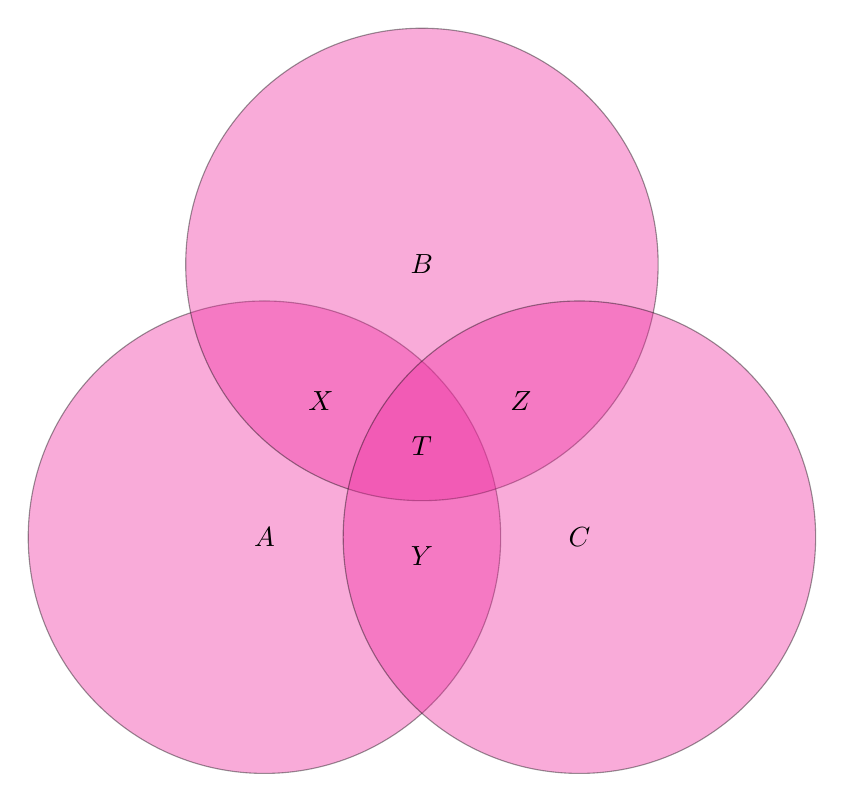
\begin{tikzpicture}[set/.style = {draw,
    circle,
    minimum size = 6cm,
    fill=Rhodamine,
    opacity = 0.4,
    text opacity = 1}]
 
\node (A) [set] {$A$};
\node (B) at (60:4cm) [set] {$B$};
\node (C) at (0:4cm) [set] {$C$};
 
\node at (barycentric cs:A=1,B=1) [left] {$X$};
\node at (barycentric cs:A=1,C=1) [below] {$Y$};
\node at (barycentric cs:B=1,C=1) [right] {$Z$};
\node at (barycentric cs:A=1,B=1,C=1) [] {$T$};
 
\end{tikzpicture}
\end{center}

\textbf{Le problème :} Si on additionne simplement $|A| + |B| + |C|$, on compte certaines zones plusieurs fois :
\begin{itemize}
    \item Les intersections deux à deux ($X$, $Y$, $Z$) sont comptées \textbf{deux fois}
    \item L'intersection triple ($T$) est comptée \textbf{trois fois}
\end{itemize}

\textbf{La solution :} On corrige en soustrayant les intersections deux à deux, mais alors l'intersection triple est comptée :
\begin{itemize}
    \item $+3$ fois dans la somme initiale
    \item $-3$ fois dans la soustraction des intersections deux à deux (car elle appartient à chacune)
    \item Donc $0$ fois au total ! Il faut la rajouter.
\end{itemize}

D'où la formule : $|A \cup B \cup C| = |A| + |B| + |C| - |A \cap B| - |A \cap C| - |B \cap C| + |A \cap B \cap C|$
\end{intuitionbox}

Ce que nous avons fait visuellement pour 3 ensembles peut être généralisé par récurrence à $n$ ensembles. La formule générale suit le même principe d'alternance des signes :

\begin{theorembox}[Principe d'Inclusion-Exclusion généralisé]
Pour $n$ ensembles finis $A_1, A_2, \dots, A_n$, on a :
\begin{align*}
|A_1 \cup A_2 \cup \cdots \cup A_n| = & \sum_{i=1}^n |A_i| \\
& - \sum_{1 \leq i < j \leq n} |A_i \cap A_j| \\
& + \sum_{1 \leq i < j < k \leq n} |A_i \cap A_j \cap A_k| \\
& - \cdots \\
& + (-1)^{n+1} |A_1 \cap A_2 \cap \cdots \cap A_n|
\end{align*}
Ce qui s'écrit plus compactement :
$$ \left| \bigcup_{i=1}^n A_i \right| = \sum_{k=1}^n (-1)^{k+1} \sum_{1 \leq i_1 < i_2 < \cdots < i_k \leq n} |A_{i_1} \cap A_{i_2} \cap \cdots \cap A_{i_k}| $$
\end{theorembox}

% NOUVEAU :
La preuve formelle que cette formule gigantesque fonctionne est fascinante. Il suffit de montrer que n'importe quel élément $x$ de l'union, peu importe à combien d'ensembles il appartient, est compté \textbf{exactement une fois} au final.
% FIN NOUVEAU

\begin{proofbox}[Preuve par comptage d'un élément]
Considérons un élément $x$ qui appartient à exactement $k$ ensembles parmi les $n$ ensembles $A_1, \ldots, A_n$ (où $k \ge 1$). Nous devons montrer que $x$ est compté exactement 1 fois par la formule.

Analysons combien de fois $x$ est compté dans chaque somme de la formule :
\begin{itemize}
    \item \textbf{Première somme ($\sum |A_i|$)} : $x$ est dans $k$ ensembles, donc il est ajouté $k$ fois. Le nombre de fois est $\binom{k}{1}$.
    
    \item \textbf{Deuxième somme ($-\sum |A_i \cap A_j|$)} : $x$ est compté (et soustrait) pour chaque \textit{paire} d'ensembles auxquels il appartient. Comme il appartient à $k$ ensembles, il y a $\binom{k}{2}$ telles paires.
    
    \item \textbf{Troisième somme ($+\sum |A_i \cap A_j \cap A_k|$)} : $x$ est ajouté pour chaque \textit{triplet} d'ensembles auxquels il appartient. Il y en a $\binom{k}{3}$.
    
    \item \textbf{Et ainsi de suite...}
\end{itemize}
Au total, l'élément $x$ est compté :
$$ \text{Total} = \binom{k}{1} - \binom{k}{2} + \binom{k}{3} - \cdots + (-1)^{k-1}\binom{k}{k} \text{ fois.} $$
Pour évaluer cette somme, rappelons l'identité fondamentale du binôme de Newton :
$$ (1 + x)^k = \sum_{j=0}^{k} \binom{k}{j} x^j = \binom{k}{0} + \binom{k}{1}x + \binom{k}{2}x^2 + \cdots $$
Si nous posons $x = -1$, nous obtenons :
$$ (1-1)^k = 0 = \binom{k}{0} - \binom{k}{1} + \binom{k}{2} - \binom{k}{3} + \cdots + (-1)^k\binom{k}{k} $$
Sachant que $\binom{k}{0} = 1$, on a :
$$ 0 = 1 - \left( \binom{k}{1} - \binom{k}{2} + \binom{k}{3} - \cdots + (-1)^{k-1}\binom{k}{k} \right) $$
En réarrangeant, on trouve :
$$ 1 = \binom{k}{1} - \binom{k}{2} + \binom{k}{3} - \cdots + (-1)^{k-1}\binom{k}{k} $$
Cela prouve que n'importe quel élément de l'union est compté exactement une fois.
\end{proofbox}

Ce principe est très utile en probabilité, car il permet de calculer $P(A \cup B \cup \dots)$ en se basant sur les probabilités des intersections, qui sont souvent plus faciles à trouver.

\begin{examplebox}[Application probabiliste]
On lance trois dés équilibrés. Quelle est la probabilité d'obtenir au moins un 6 ?

\textbf{Solution avec inclusion-exclusion :}

Soit $A$ = "le premier dé montre 6", $B$ = "le deuxième dé montre 6", $C$ = "le troisième dé montre 6".

On veut $P(A \cup B \cup C)$.

\begin{align*}
P(A \cup B \cup C) &= P(A) + P(B) + P(C) \\
&\quad - P(A \cap B) - P(A \cap C) - P(B \cap C) \\
&\quad + P(A \cap B \cap C) \\
&= \frac{1}{6} + \frac{1}{6} + \frac{1}{6} - \frac{1}{36} - \frac{1}{36} - \frac{1}{36} + \frac{1}{216} \\
&= \frac{3}{6} - \frac{3}{36} + \frac{1}{216} = \frac{1}{2} - \frac{1}{12} + \frac{1}{216} \\
&= \frac{108 - 18 + 1}{216} = \frac{91}{216} \approx 0.421
\end{align*}

\textbf{Vérification par la méthode complémentaire :}

La probabilité de n'obtenir aucun 6 est $\left(\frac{5}{6}\right)^3 = \frac{125}{216}$, donc la probabilité d'au moins un 6 est $1 - \frac{125}{216} = \frac{91}{216}$.
\end{examplebox}

\subsection{Exercices}

Cette série d'exercices vise à renforcer votre compréhension des concepts fondamentaux du dénombrement et de la probabilité naïve. La difficulté augmente progressivement.

% --- Concepts de Base et Probabilité Naïve ---

\begin{exercicebox}[Exercice 1 : Univers et Événements]
On lance deux dés à 6 faces, un rouge et un bleu.
\begin{enumerate}
    \item Décrivez l'univers $S$ de cette expérience. Quelle est sa taille $|S|$ ?
    \item Soit $A$ l'événement "la somme des dés est égale à 7". Listez les issues appartenant à $A$. Calculez $P(A)$.
    \item Soit $B$ l'événement "le dé rouge montre un 3". Listez les issues appartenant à $B$. Calculez $P(B)$.
    \item Décrivez l'événement $A \cap B$ et calculez sa probabilité.
\end{enumerate}
\end{exercicebox}

\begin{exercicebox}[Exercice 2 : Tirage de Cartes (Prob. Naïve)]
On tire une carte au hasard d'un jeu standard de 52 cartes.
\begin{enumerate}
    \item Quelle est la probabilité de tirer un Roi ?
    \item Quelle est la probabilité de tirer une carte rouge (Cœur ou Carreau) ?
    \item Quelle est la probabilité de tirer une figure (Valet, Dame, Roi) ?
    \item Quelle est la probabilité de tirer un As rouge ?
\end{enumerate}
\end{exercicebox}

\begin{exercicebox}[Exercice 3 : Urne Simple (Prob. Naïve)]
Une urne contient 5 boules rouges, 3 boules bleues et 2 boules vertes. On tire une boule au hasard.
\begin{enumerate}
    \item Quelle est la probabilité qu'elle soit bleue ?
    \item Quelle est la probabilité qu'elle ne soit pas verte ?
\end{enumerate}
\end{exercicebox}

% --- Permutations ---

\begin{exercicebox}[Exercice 4 : Anagrammes (Permutation Simple)]
Combien d'anagrammes distinctes peut-on former avec les lettres du mot "MATHS" ?
\end{exercicebox}

\begin{exercicebox}[Exercice 5 : Course (Arrangement)]
Dix athlètes participent à une course. Combien y a-t-il de classements possibles pour les 3 premières places (médaille d'or, d'argent, de bronze) ?
\end{exercicebox}

\begin{exercicebox}[Exercice 6 : Anagrammes (Permutation avec Répétition)]
Combien d'anagrammes distinctes peut-on former avec les lettres du mot "PROBABILITE" ?
\end{exercicebox}

% --- Combinaisons ---

\begin{exercicebox}[Exercice 7 : Choix d'un Comité (Combinaison)]
Une classe compte 15 étudiants. De combien de manières peut-on choisir un comité de 4 étudiants ?
\end{exercicebox}

\begin{exercicebox}[Exercice 8 : Mains de Poker (Combinaison)]
Dans un jeu de 52 cartes, combien de "mains" de 5 cartes différentes peut-on former ?
\end{exercicebox}

\begin{exercicebox}[Exercice 9 : Comité Mixte (Combinaison)]
À partir d'un groupe de 6 hommes et 4 femmes, combien de comités de 3 personnes peut-on former contenant exactement 2 hommes et 1 femme ?
\end{exercicebox}

\begin{exercicebox}[Exercice 10 : Probabilité avec Combinaisons]
On tire simultanément 3 cartes d'un jeu de 52 cartes. Quelle est la probabilité d'obtenir exactement 2 Rois ?
\end{exercicebox}

% --- Combinaisons avec Répétition (Étoiles et Bâtons) ---

\begin{exercicebox}[Exercice 11 : Distribution de Bonbons (Étoiles et Bâtons)]
De combien de manières peut-on distribuer 8 bonbons identiques à 3 enfants ? (Certains enfants peuvent ne rien recevoir).
\end{exercicebox}

\begin{exercicebox}[Exercice 12 : Solutions d'Équation (Étoiles et Bâtons)]
Combien y a-t-il de solutions entières non négatives ($x_i \ge 0$) à l'équation $x_1 + x_2 + x_3 + x_4 = 10$ ?
\end{exercicebox}

\begin{exercicebox}[Exercice 13 : Distribution avec Minimum (Étoiles et Bâtons avec Contrainte)]
De combien de manières peut-on distribuer 12 pommes identiques à 4 enfants, si chaque enfant doit recevoir au moins une pomme ?
\end{exercicebox}

% --- Principe d'Inclusion-Exclusion ---

\begin{exercicebox}[Exercice 14 : Divisibilité (Inclusion-Exclusion 2 Ensembles)]
Parmi les entiers de 1 à 100, combien sont divisibles par 2 OU par 3 ?
\end{exercicebox}

\begin{exercicebox}[Exercice 15 : Langues (Inclusion-Exclusion 2 Ensembles)]
Dans un groupe de 50 étudiants, 30 étudient l'anglais, 25 étudient l'espagnol et 10 étudient les deux langues. Combien d'étudiants étudient au moins une de ces deux langues ? Combien n'en étudient aucune ?
\end{exercicebox}

\begin{exercicebox}[Exercice 16 : Divisibilité (Inclusion-Exclusion 3 Ensembles)]
Parmi les entiers de 1 à 100, combien sont divisibles par 2, 3 OU 5 ?
\end{exercicebox}

% --- Problèmes Combinés et Plus Difficiles ---

\begin{exercicebox}[Exercice 17 : Chemins sur un Grillage (Combinaison)]
Sur un grillage, combien y a-t-il de chemins pour aller du point (0,0) au point (4,3) en se déplaçant uniquement vers la droite (D) ou vers le haut (H) ?
\end{exercicebox}

\begin{exercicebox}[Exercice 18 : Probabilité Hypergéométrique]
Une urne contient 7 boules blanches et 5 boules noires. On tire successivement et sans remise 4 boules. Quelle est la probabilité d'obtenir 2 blanches et 2 noires ?
\end{exercicebox}

\begin{exercicebox}[Exercice 19 : Arrangement Circulaire]
De combien de manières 6 personnes peuvent-elles s'asseoir autour d'une table ronde ? (Deux arrangements sont considérés identiques si chaque personne a les mêmes voisins).
\end{exercicebox}

\begin{exercicebox}[Exercice 20 : Problème des Dérangements (Inclusion-Exclusion)]
Quatre lettres sont adressées à quatre personnes différentes, avec les enveloppes correspondantes. On met chaque lettre au hasard dans une enveloppe. Quelle est la probabilité qu'\textit{aucune} lettre ne soit dans la bonne enveloppe ?
\end{exercicebox}



\subsection{Corrections des Exercices}

% --- Corrections : Concepts de Base et Probabilité Naïve ---

\begin{correctionbox}[Correction Exercice 1 : Univers et Événements]
1) L'univers $S$ est l'ensemble de toutes les paires $(r, b)$ où $r$ est le résultat du dé rouge et $b$ celui du dé bleu. $S = \{ (1,1), (1,2), \dots, (1,6), (2,1), \dots, (6,6) \}$. La taille de l'univers est $|S| = 6 \times 6 = 36$.

2) L'événement $A$ (somme égale à 7) est $A = \{ (1,6), (2,5), (3,4), (4,3), (5,2), (6,1) \}$. Il y a $|A|=6$ issues favorables. La probabilité est $P(A) = |A|/|S| = 6/36 = 1/6$.

3) L'événement $B$ (dé rouge montre 3) est $B = \{ (3,1), (3,2), (3,3), (3,4), (3,5), (3,6) \}$. Il y a $|B|=6$ issues favorables. La probabilité est $P(B) = |B|/|S| = 6/36 = 1/6$.

4) L'événement $A \cap B$ est l'ensemble des issues où la somme est 7 ET le dé rouge est 3. La seule issue possible est $(3,4)$. Donc $A \cap B = \{ (3,4) \}$. La probabilité est $P(A \cap B) = |A \cap B|/|S| = 1/36$.
\end{correctionbox}

\begin{correctionbox}[Correction Exercice 2 : Tirage de Cartes (Prob. Naïve)]
Le nombre total d'issues est $|S| = 52$.

a) Il y a 4 Rois. $P(\text{Roi}) = 4/52 = 1/13$.

b) Il y a 26 cartes rouges (13 Cœurs + 13 Carreaux). $P(\text{Rouge}) = 26/52 = 1/2$.

c) Il y a 12 figures (4 Valets + 4 Dames + 4 Rois). $P(\text{Figure}) = 12/52 = 3/13$.

d) Il y a 2 As rouges (As de Cœur, As de Carreau). $P(\text{As Rouge}) = 2/52 = 1/26$.
\end{correctionbox}

\begin{correctionbox}[Correction Exercice 3 : Urne Simple (Prob. Naïve)]
Le nombre total de boules est $5+3+2 = 10$.

a) Il y a 3 boules bleues. $P(\text{Bleue}) = 3/10$.

b) L'événement "ne pas être verte" est le complémentaire de "être verte". Il y a 2 boules vertes, donc $P(\text{Verte}) = 2/10$. La probabilité cherchée est $P(\text{Non Verte}) = 1 - P(\text{Verte}) = 1 - 2/10 = 8/10 = 4/5$. (Alternativement, il y a $5+3=8$ boules non vertes, donc $P=8/10$).
\end{correctionbox}

% --- Corrections : Permutations ---

\begin{correctionbox}[Correction Exercice 4 : Anagrammes (Permutation Simple)]
Le mot "MATHS" a 5 lettres distinctes. Le nombre d'anagrammes est le nombre de permutations de ces 5 lettres, soit $5! = 5 \times 4 \times 3 \times 2 \times 1 = 120$.
\end{correctionbox}

\begin{correctionbox}[Correction Exercice 5 : Course (Arrangement)]
On cherche le nombre de façons d'ordonner 3 athlètes parmi 10. C'est un arrangement (permutation de $k$ parmi $n$) :
$P(10, 3) = \frac{10!}{(10-3)!} = \frac{10!}{7!} = 10 \times 9 \times 8 = 720$.
Il y a 720 podiums possibles.
\end{correctionbox}

\begin{correctionbox}[Correction Exercice 6 : Anagrammes (Permutation avec Répétition)]
Le mot "PROBABILITE" a 11 lettres. Les répétitions sont : B (2 fois), I (2 fois). Les autres lettres (P, R, O, A, L, T, E) apparaissent une fois.
Le nombre d'anagrammes distinctes est :
$$ \frac{11!}{2! \times 2!} = \frac{39,916,800}{2 \times 2} = \frac{39,916,800}{4} = 9,979,200 $$
\end{correctionbox}

% --- Corrections : Combinaisons ---

\begin{correctionbox}[Correction Exercice 7 : Choix d'un Comité (Combinaison)]
L'ordre ne compte pas, c'est donc une combinaison de 4 étudiants parmi 15 :
$$ \binom{15}{4} = \frac{15!}{4!(15-4)!} = \frac{15!}{4!11!} = \frac{15 \times 14 \times 13 \times 12}{4 \times 3 \times 2 \times 1} = 15 \times 7 \times 13 \times 1 = 1365 $$
Il y a 1365 comités possibles.
\end{correctionbox}

\begin{correctionbox}[Correction Exercice 8 : Mains de Poker (Combinaison)]
On choisit 5 cartes parmi 52, sans ordre. C'est une combinaison :
$$ \binom{52}{5} = \frac{52!}{5!(52-5)!} = \frac{52!}{5!47!} = \frac{52 \times 51 \times 50 \times 49 \times 48}{5 \times 4 \times 3 \times 2 \times 1} = 2,598,960 $$
Il y a 2,598,960 mains de poker possibles.
\end{correctionbox}

\begin{correctionbox}[Correction Exercice 9 : Comité Mixte (Combinaison, Principe Multiplicatif)]
Il faut choisir 2 hommes parmi 6 ET 1 femme parmi 4. On multiplie les possibilités pour chaque choix :
Nombre de façons = (choix des hommes) $\times$ (choix des femmes)
$$ = \binom{6}{2} \times \binom{4}{1} = \frac{6 \times 5}{2 \times 1} \times \frac{4}{1} = 15 \times 4 = 60 $$
Il y a 60 comités possibles.
\end{correctionbox}

\begin{correctionbox}[Correction Exercice 10 : Probabilité avec Combinaisons]
L'univers $S$ est l'ensemble de toutes les mains de 3 cartes. $|S| = \binom{52}{3}$.
L'événement $A$ est "obtenir exactement 2 Rois". Pour cela, il faut choisir 2 Rois parmi les 4 Rois ET 1 carte qui n'est pas un Roi parmi les 48 autres cartes.
$|A| = \binom{4}{2} \times \binom{48}{1}$.
La probabilité est $P(A) = \frac{|A|}{|S|} = \frac{\binom{4}{2} \binom{48}{1}}{\binom{52}{3}}$.
$$ P(A) = \frac{\frac{4 \times 3}{2 \times 1} \times 48}{\frac{52 \times 51 \times 50}{3 \times 2 \times 1}} = \frac{6 \times 48}{22100} = \frac{288}{22100} \approx 0.013 $$
\end{correctionbox}

% --- Corrections : Combinaisons avec Répétition (Étoiles et Bâtons) ---

\begin{correctionbox}[Correction Exercice 11 : Distribution de Bonbons (Étoiles et Bâtons)]
C'est un problème de distribution de $k=8$ objets identiques (bonbons) dans $n=3$ boîtes distinctes (enfants). On utilise la formule $\binom{n+k-1}{k}$.
Nombre de manières = $\binom{3+8-1}{8} = \binom{10}{8} = \binom{10}{2} = \frac{10 \times 9}{2 \times 1} = 45$.
\end{correctionbox}

\begin{correctionbox}[Correction Exercice 12 : Solutions d'Équation (Étoiles et Bâtons)]
Cela revient à distribuer $k=10$ unités identiques dans $n=4$ variables distinctes.
Nombre de solutions = $\binom{n+k-1}{k} = \binom{4+10-1}{10} = \binom{13}{10} = \binom{13}{3} = \frac{13 \times 12 \times 11}{3 \times 2 \times 1} = 286$.
\end{correctionbox}

\begin{correctionbox}[Correction Exercice 13 : Distribution avec Minimum (Étoiles et Bâtons avec Contrainte)]
On doit distribuer $k=12$ pommes à $n=4$ enfants, avec $x_i \ge 1$.
On commence par donner une pomme à chaque enfant. Il reste $12 - 4 = 8$ pommes à distribuer sans contrainte (les $x'_i$ peuvent être nuls).
Le problème devient : distribuer $k'=8$ pommes à $n=4$ enfants.
Nombre de manières = $\binom{n+k'-1}{k'} = \binom{4+8-1}{8} = \binom{11}{8} = \binom{11}{3} = \frac{11 \times 10 \times 9}{3 \times 2 \times 1} = 165$.
\end{correctionbox}

% --- Corrections : Principe d'Inclusion-Exclusion ---

\begin{correctionbox}[Correction Exercice 14 : Divisibilité (Inclusion-Exclusion 2 Ensembles)]
Soit $A$ l'ensemble des entiers $\le 100$ divisibles par 2, et $B$ l'ensemble des entiers $\le 100$ divisibles par 3. On cherche $|A \cup B|$.
$|A| = \lfloor 100/2 \rfloor = 50$.
$|B| = \lfloor 100/3 \rfloor = 33$.
$|A \cap B|$ = ensemble des entiers divisibles par $2 \times 3 = 6$. $|A \cap B| = \lfloor 100/6 \rfloor = 16$.
Par inclusion-exclusion : $|A \cup B| = |A| + |B| - |A \cap B| = 50 + 33 - 16 = 67$.
\end{correctionbox}

\begin{correctionbox}[Correction Exercice 15 : Langues (Inclusion-Exclusion 2 Ensembles)]
Soit $E$ l'ensemble des étudiants étudiant l'anglais, $S$ l'ensemble de ceux étudiant l'espagnol.
$|E| = 30$, $|S| = 25$, $|E \cap S| = 10$.
Nombre d'étudiants étudiant au moins une langue : $|E \cup S| = |E| + |S| - |E \cap S| = 30 + 25 - 10 = 45$.
Nombre total d'étudiants = 50.
Nombre d'étudiants n'étudiant aucune de ces langues = Total - $|E \cup S| = 50 - 45 = 5$.
\end{correctionbox}

\begin{correctionbox}[Correction Exercice 16 : Divisibilité (Inclusion-Exclusion 3 Ensembles)]
Soit $A_2, A_3, A_5$ les ensembles des entiers $\le 100$ divisibles respectivement par 2, 3, 5. On cherche $|A_2 \cup A_3 \cup A_5|$.
$|A_2|=50$, $|A_3|=33$, $|A_5|=20$.
$|A_2 \cap A_3| = |A_6| = \lfloor 100/6 \rfloor = 16$.
$|A_2 \cap A_5| = |A_{10}| = \lfloor 100/10 \rfloor = 10$.
$|A_3 \cap A_5| = |A_{15}| = \lfloor 100/15 \rfloor = 6$.
$|A_2 \cap A_3 \cap A_5| = |A_{30}| = \lfloor 100/30 \rfloor = 3$.
Par inclusion-exclusion :
$|A_2 \cup A_3 \cup A_5| = (|A_2|+|A_3|+|A_5|) - (|A_2 \cap A_3|+|A_2 \cap A_5|+|A_3 \cap A_5|) + |A_2 \cap A_3 \cap A_5|$
$= (50+33+20) - (16+10+6) + 3 = 103 - 32 + 3 = 74$.
\end{correctionbox}

% --- Corrections : Problèmes Combinés et Plus Difficiles ---

\begin{correctionbox}[Correction Exercice 17 : Chemins sur un Grillage (Combinaison)]
Pour aller de (0,0) à (4,3), il faut faire un total de $4+3=7$ déplacements. Parmi ces 7 déplacements, il faut choisir les 4 moments où l'on va à droite (les 3 autres seront obligatoirement vers le haut), ou choisir les 3 moments où l'on va vers le haut.
Le nombre de chemins est $\binom{7}{4} = \binom{7}{3} = \frac{7 \times 6 \times 5}{3 \times 2 \times 1} = 35$.
\end{correctionbox}

\begin{correctionbox}[Correction Exercice 18 : Probabilité Hypergéométrique]
C'est un tirage sans remise. On peut utiliser la loi hypergéométrique ou le dénombrement.
Population totale = $7+5=12$ boules. On en tire $m=4$.
On veut $k=2$ blanches (parmi $w=7$) et $m-k=2$ noires (parmi $b=5$).
Probabilité = $\frac{\binom{w}{k} \binom{b}{m-k}}{\binom{w+b}{m}} = \frac{\binom{7}{2} \binom{5}{2}}{\binom{12}{4}}$.
$$ P = \frac{(\frac{7 \times 6}{2}) \times (\frac{5 \times 4}{2})}{(\frac{12 \times 11 \times 10 \times 9}{4 \times 3 \times 2 \times 1})} = \frac{21 \times 10}{495} = \frac{210}{495} = \frac{14}{33} \approx 0.424 $$
\end{correctionbox}

\begin{correctionbox}[Correction Exercice 19 : Arrangement Circulaire]
Pour $n$ objets distincts, le nombre d'arrangements circulaires est $(n-1)!$.
Ici, $n=6$. Le nombre de manières est $(6-1)! = 5! = 120$.
L'idée est de fixer une personne, puis d'arranger les 5 autres par rapport à elle.
\end{correctionbox}

\begin{correctionbox}[Correction Exercice 20 : Problème des Dérangements (Inclusion-Exclusion)]
On cherche le nombre de dérangements de 4 éléments, noté $D_4$ ou $!4$. La probabilité sera $D_4 / 4!$.
La formule générale des dérangements (obtenue par inclusion-exclusion) est $D_n = n! \sum_{i=0}^n \frac{(-1)^i}{i!}$.
Pour $n=4$:
$D_4 = 4! (1/0! - 1/1! + 1/2! - 1/3! + 1/4!)$
$D_4 = 24 (1 - 1 + 1/2 - 1/6 + 1/24)$
$D_4 = 24 (1/2 - 1/6 + 1/24) = 24 (12/24 - 4/24 + 1/24) = 24 (9/24) = 9$.
Il y a 9 dérangements possibles sur un total de $4! = 24$ permutations.
La probabilité est $P(\text{aucun match}) = D_4 / 4! = 9/24 = 3/8 = 0.375$.
\end{correctionbox}